\documentclass[12pt,]{article}
\usepackage{lmodern}
\usepackage{amssymb,amsmath}
\usepackage{ifxetex,ifluatex}
\usepackage{fixltx2e} % provides \textsubscript
\ifnum 0\ifxetex 1\fi\ifluatex 1\fi=0 % if pdftex
  \usepackage[T1]{fontenc}
  \usepackage[utf8]{inputenc}
\else % if luatex or xelatex
  \ifxetex
    \usepackage{mathspec}
  \else
    \usepackage{fontspec}
  \fi
  \defaultfontfeatures{Ligatures=TeX,Scale=MatchLowercase}
    \setmainfont[]{Arial}
\fi
% use upquote if available, for straight quotes in verbatim environments
\IfFileExists{upquote.sty}{\usepackage{upquote}}{}
% use microtype if available
\IfFileExists{microtype.sty}{%
\usepackage{microtype}
\UseMicrotypeSet[protrusion]{basicmath} % disable protrusion for tt fonts
}{}
\usepackage[margin=.5in]{geometry}
\usepackage{hyperref}
\hypersetup{unicode=true,
            pdftitle={Group 8 Final Report},
            pdfauthor={Jingnan Bai, Kexin Wang, Yiming Miao, Qiyu Huang},
            pdfborder={0 0 0},
            breaklinks=true}
\urlstyle{same}  % don't use monospace font for urls
\usepackage{natbib}
\bibliographystyle{plainnat}
\usepackage{longtable,booktabs}
\usepackage{graphicx}
\makeatletter
\def\maxwidth{\ifdim\Gin@nat@width>\linewidth\linewidth\else\Gin@nat@width\fi}
\def\maxheight{\ifdim\Gin@nat@height>\textheight\textheight\else\Gin@nat@height\fi}
\makeatother
% Scale images if necessary, so that they will not overflow the page
% margins by default, and it is still possible to overwrite the defaults
% using explicit options in \includegraphics[width, height, ...]{}
\setkeys{Gin}{width=\maxwidth,height=\maxheight,keepaspectratio}
\IfFileExists{parskip.sty}{%
\usepackage{parskip}
\setlength{\parskip}{8pt plus 2pt minus 1pt}
}{% else
\setlength{\parindent}{0pt}
\setlength{\parskip}{8pt plus 2pt minus 1pt}
}
\setlength{\emergencystretch}{3em}  % prevent overfull lines
\providecommand{\tightlist}{%
  \setlength{\itemsep}{0pt}\setlength{\parskip}{0pt}}
\setcounter{secnumdepth}{5}

%%% Use protect on footnotes to avoid problems with footnotes in titles
\let\rmarkdownfootnote\footnote%
\def\footnote{\protect\rmarkdownfootnote}


  \title{Group 8 Final Report}
    \author{Jingnan Bai, Kexin Wang, Yiming Miao, Qiyu Huang}
      \date{2024-05-09}


%%%%%%%%%%
% personal preamble edits here
%%%%%%%%%%
\pagenumbering{gobble}

% can toggle this for Helvetica
%\usepackage{helvet}
%\renewcommand{\familydefault}{\sfdefault}

% \titlespacing*{\paragraph}{0pt}{2pt}{1em}

% set section numbering/lettering
% tips for seccntformat: https://tex.stackexchange.com/questions/95896/how-to-format-subsection-title-without-packages
\makeatletter
\def\@seccntformat#1{%
  \expandafter\ifx\csname c@#1\endcsname\c@section\else
  \expandafter\ifx\csname c@#1\endcsname\c@paragraph\else
  \csname the#1\endcsname\quad
  \fi\fi}
  
  % stucture for these commands: https://texfaq.org/FAQ-atsigns
  \renewcommand\section{
  \@startsection{section}{1}{\z@}
    {-3.5ex \@plus -1ex \@minus -.2ex}
    {1.0ex \@plus.2ex} %reduce space below section (was 1.5ex)
    {\normalfont\normalsize\bf\uppercase}} %modify font style
    
  \renewcommand\subsection{
  \@startsection{subsection}{2}{\z@}
    {-1.5ex\@plus -1ex \@minus -.2ex}%reduce space above subsection (was -3.25ex)
    {0.5ex \@plus .2ex}%reduce space below subsection (was 1.5ex)
    {\normalfont\normalsize\bf}} %modify font style
    
  \renewcommand\subsubsection{
  \@startsection{subsubsection}{3}{\z@}
    {-1.0ex\@plus -1ex \@minus -.2ex}%reduce space above subsubsection (was -3.25ex)
    {0.5ex \@plus .2ex}%reduce space below subsubsection (was 1.5ex)
    {\normalfont\normalsize\bf}} %modify font style
    
  \renewcommand\paragraph{
  \@startsection{paragraph}{4}{\z@}
    {-0.5ex\@plus -1ex \@minus -.2ex}%reduce space above paragraph (was -3.25ex)
    {-1.5ex \@plus .2ex}%convert space below paragraph to an indent (was 1.5ex)
    {\normalfont\normalsize\bf}} %modify font style    
\makeatother

\renewcommand\thesubsection{\Alph{subsection}.}
\renewcommand\thesubsubsection{\thesubsection\arabic{subsubsection}.}

% reduce spacing at the top of lists
\usepackage{enumitem}
\setlist{topsep = 2pt}

% allow text to wrap around figures
\usepackage{graphicx}
\usepackage{wrapfig}

%%%%%%%%%%

\begin{document}
\maketitle

\hypertarget{introduction}{%
\section{Introduction}\label{introduction}}

Parkinson's disease (PD) ranks as the second-most common
neurodegenerative disorder in the US, affecting nearly 90,000
individuals annually. Characterized by uncontrollable movements such as
shaking, stiffness, and imbalance, PD significantly diminishes patients'
quality of life. Characterized as a progressive neurological disorder,
PD occurs due to the gradual degeneration or death of nerve cells in the
basal ganglia. The exact cause of neuronal death remains inconclusive,
though current research suggests a combination of specific genetic
variants and environmental factors, including toxin exposure, as leading
risk contributors.

Parkinson's disease (PD) is a progressive neurological disorder that
develops over time as a result of nerve cells in the basal ganglia
gradually degenerating or dying. Although the precise cause of neuronal
death is still unknown, recent research points to a combination of toxin
exposure and particular genetic variants as the main risk factors.

Due to the significant consequences of Parkinson's disease, our group
has decided to look into the underlying characteristics and create a
predictive model for an early diagnosis. This research plays a critical
role in raising the standard of patient care by enabling medical
professionals to create customized treatment regimens that improve
patients' quality of life.

Our research also aims to facilitate early detection, which can slow the
progression of the disease and greatly increase the opportunities for
intervention. Our research may help develop preventive public health
initiatives by pinpointing particular lifestyle factors associated with
Parkinson's, which could lower the overall incidence of Parkinson's
disease. These initiatives demonstrate how crucially important our
project is to improving Parkinson's disease patient care and medical
knowledge.

\hypertarget{specific-aims}{%
\section{Specific Aims}\label{specific-aims}}

A. Specific Aim 1

Aim 1 of our study is to investigate Key Inferences for Pre-Diagnostic
and Post-Diagnostic PD Patients. This initial aim is crucial as it sets
the foundation for developing effective diagnostic tools and
interventions. By identifying specific characteristics or markers that
are significantly associated with Parkinson's disease, we can enhance
our understanding of its pathophysiology and possibly find new targets
for treatment intervention.

B. Specific Aim 2

Aim 2 of our study is to develop a predictive model for the early
diagnosis of Parkinson's disease (PD) using a wealth of physiological,
lifestyle, and demographic data from the UK Biobank. This goal involves
investigating participant data on their trunks and limbs among other
things in order to create a model that can accurately predict the onset
of Parkinson's disease (PD) in its early stages.

\hypertarget{rationale}{%
\section{Rationale}\label{rationale}}

A. Significance

Data analysis related to Parkinson's disease (PD) is crucial for
improving our knowledge of this severe neurodegenerative condition.
Researchers can find subtle patterns and correlations between genetic,
environmental, and lifestyle factors that influence the development and
progression of Parkinson's disease (PD) by carefully examining data
related to the disease. The development of predictive models that can
identify people at increased risk much earlier than is currently
feasible will require this deeper understanding. The management of
Parkinson's disease (PD) depends heavily on early detection because it
enables the implementation of interventions that may significantly alter
the course of the disease, possibly delaying the beginning of severe
symptoms and extending patient independence.

In addition, the examination of Parkinson's disease data makes it easier
to identify particular biomarkers that can be used for both continuous
disease monitoring and early detection. This ability increases the
efficacy of therapeutic interventions by enabling more precise
modification of treatment plans to meet the specific requirements of
patients. Furthermore, information gathered from PD data analysis plays
an essential part in illuminating the basic processes underlying
Parkinson's disease. This information is essential for the creation of
novel remedies and treatments that concentrate on these fundamental
mechanisms.

B. Innovation

Because of the skewed nature of our dataset---in which the number of
healthy individuals is significantly greater than that of PD
patients---our research on Parkinson's disease (PD) presents a special
set of challenges. This imbalance may result in skewed analyses and less
reliable findings. In order to creatively address this problem, our
research makes use of multiple advanced methods to efficiently balance
the dataset. To create synthetic data, we use techniques like WOE and
NMS algorithms. By assisting in the normalization of the dataset
distribution, these methods improve the precision and representativeness
of our analysis concerning the actual effects of Parkinson's disease.
Our diligent approach to settle this imbalance strengthens the basis for
PD research going forward, guaranteeing that the knowledge acquired is
legitimate and applicable.

\hypertarget{research-plan}{%
\section{Research Plan}\label{research-plan}}

Our research on Parkinson's disease (PD) is structured into a three-step
plan designed for maximum efficiency and clarity, ensuring a thorough
investigation into the complexities of PD.

Step 1: Exploratory Data Analysis (EDA)

During the EDA phase, we delve into the dataset to understand data
structure and extract preliminary insights. This important stage directs
the course of our more in-depth research and aids in our understanding
of the data's underlying structure. At this point, we start to formulate
theories regarding the connections between the data that might be
relevant to Parkinson's disease.

Step 2: Data Processing

The initial stage of our research involves addressing the inherent
imbalance within our dataset, a common challenge in medical research,
which would be addressed with propensity score matching (PSM). We also
apply techniques such as WOE and information value for feature
filtering, while using the NMS algorithm to deal with potential
collinearity.

Step 3: Model Building and Evaluation

The final stage involves constructing predictive models using techniques
such as Logistic Regression, Mixed-effects Model, Random Forest. We
carefully evaluate these models to make sure they are able to reliably
predict PD risk and demonstrate good generalization across a wide range
of populations. This comprehensive evaluation procedure is necessary to
confirm that our models are accurate.

This research plan enables us to approach Parkinson's disease data with
precision, from initial data correction to advanced model development.
Our objective is to uncover deep understanding into the factors that
predict Parkinson's disease (PD) and to offer strong frameworks for
managing and predicting the disease by carefully navigating these steps.

\hypertarget{specific-aim-1-investigate-key-inferences-for-pre-diagnostic-and-post-diagnostic-pd-patients}{%
\section{Specific Aim 1: Investigate Key Inferences for Pre-Diagnostic
and Post-Diagnostic PD
Patients}\label{specific-aim-1-investigate-key-inferences-for-pre-diagnostic-and-post-diagnostic-pd-patients}}

\hypertarget{hypothesis}{%
\subsection{Hypothesis}\label{hypothesis}}

Patient diet (specific dietary patterns or nutritional intake), habits
(exercise frequency, tobacco use, alcohol intake), psychological
factors, and social activities may significantly affect the occurrence
of Parkinson's disease. We are going to model the characteristics of
UKBiobank participants and investigate the potential associations.

\hypertarget{rationale-1}{%
\subsection{Rationale}\label{rationale-1}}

The emphasis on these factors is due to the multifactorial nature of
Parkinson's disease, which involves complex interactions between genetic
predisposition and environmental exposures. In previous clinical
research, it has been established that specific dietary components such
as antioxidants found in fruits and vegetables can reduce oxidative
stress, which is crucial in the neurodegenerative process observed in
Parkinson's disease. While these results provide valuable information on
protective dietary elements, a key question that remains in our
understanding is how broader lifestyle patterns, including exercise,
tobacco use, and alcohol consumption, interact with dietary habits,
psychological and social factors, and demographic backgrounds to
influence the risk of Parkinson's disease.

\hypertarget{challenge-and-assumptions}{%
\subsection{Challenge and Assumptions}\label{challenge-and-assumptions}}

The UK Biobank data collection occurred in four waves: initially between
2006 and 2010, followed by subsequent collections in 2012, 2014, and
2019. The reporting dates for PD in our dataset range from 1981 to 2021,
with a median year of 2017. This temporal framework facilitates
longitudinal analysis but complicates aligning PD report dates with the
data collection phases. To address this, we separated the PD patients
into two cohorts based on their PD diagnosis status at baseline for
separate analyses:

Cohort 1: participants who were not diagnosed with PD at baseline but
received a diagnosis in subsequent follow-ups. We compared their
baseline characteristics with those of individuals without PD to
identify potential risk factors or early indicators of PD.

Cohort 2: patients who have already been diagnosed with PD at baseline
and four instances were documented after the PD report. This cohort
allows us to examine the progression of PD and its impact on quality of
life over time.

Considering all the background information, our analysis incorporated a
few assumptions. For example, we assumed that the PD diagnosis time is
accurate relative to the onset of noticeable symptoms. That is,
individuals with similar symptom severity are diagnosed within a
comparable timeframe. We also assumed that the intervals between the 4
recorded instances are comparable, disregarding various time
differences.

\hypertarget{task-1---analyze-baseline-characteristics-prior-to-pd-onset}{%
\subsection{Task 1 - Analyze baseline characteristics prior to PD
onset}\label{task-1---analyze-baseline-characteristics-prior-to-pd-onset}}

\hypertarget{participant-and-feature-selection}{%
\subsubsection{Participant and Feature
Selection}\label{participant-and-feature-selection}}

From the entire dataset comprising 1294 features across 96,512
participants, 463 were diagnosed with PD. For Cohort 1, we selected 360
participants who developed PD post-baseline, and matched the patients
with 360 healthy individuals using propensity score matching. This
matching was based on four demographic factors: age, sex, ethnicity, and
Townsend Deprivation Index.

From the initial 1,296 variables, we focused on 468 that were recorded
at baseline. Then, 201 of the 468 variables were retained, after
removing variables with a missing rate exceeding 20\%, high
correlations, and categorical variables with near zero variance. These
were then analyzed using forward stepwise selection to pinpoint critical
variables related to PD onset.

\begin{figure}
\centering
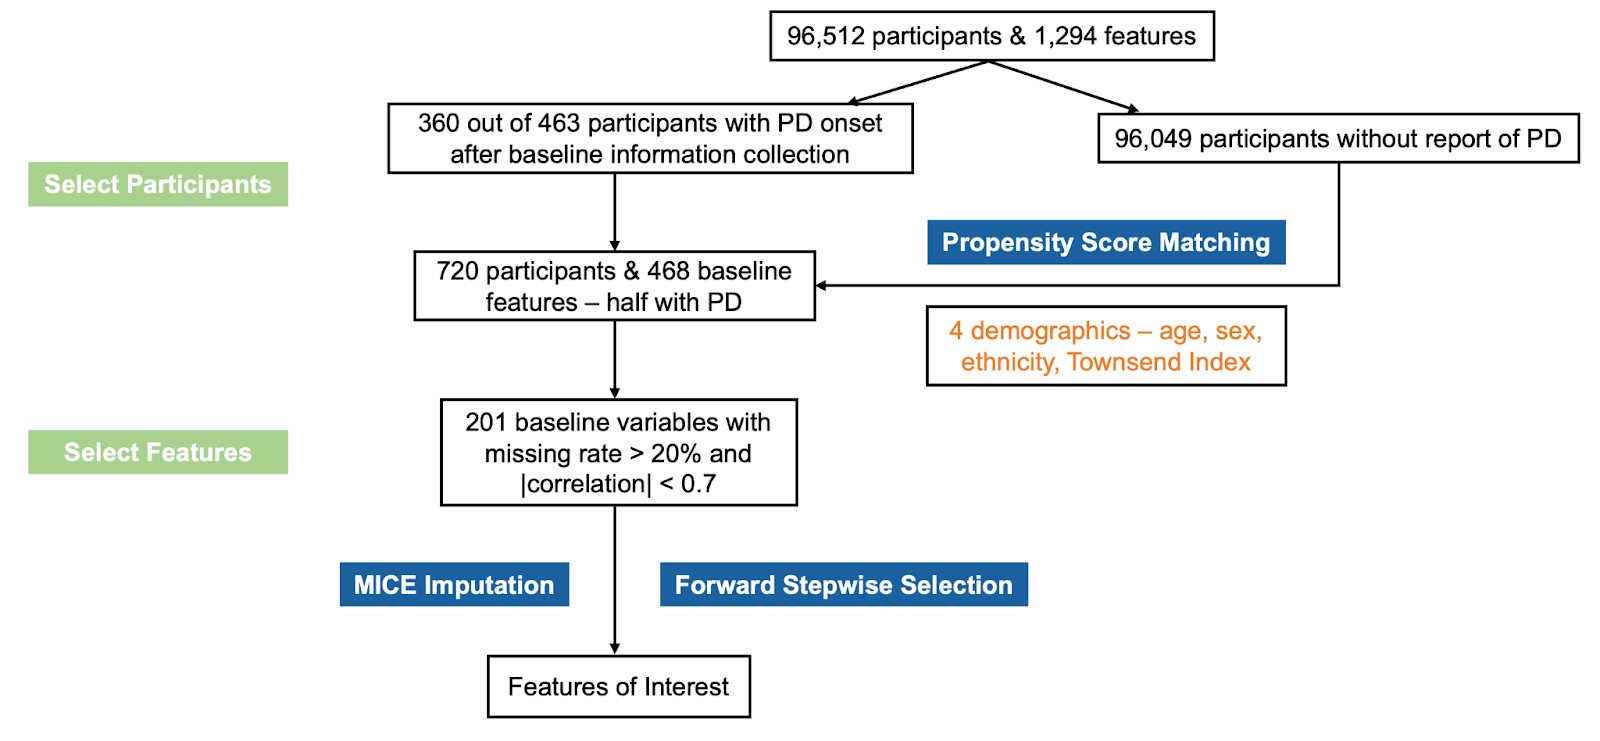
\includegraphics{../figure/Figure 1 - Workflow of Aim 1 - Task 1.png}
\caption{Workflow of Aim 1 - Task 1}
\end{figure}

\hypertarget{logistic-regression}{%
\subsubsection{Logistic Regression}\label{logistic-regression}}

Logistic regression was employed to assess the odds ratio of PD onset
given various baseline characteristics. To retain information at a
maximized level, MICE algorithm was used to impute missing data. The
final model, refined through forward stepwise selection, highlighted 46
variables, with 20 showing statistical significance.

\hypertarget{interpretation-of-results}{%
\subsubsection{Interpretation of
Results}\label{interpretation-of-results}}

Forest plot below (Figure 2) visualizes the odds ratio of statistically
significant variables. These variables generally fell into three
categories: physical activity (measured via accelerometers), lifestyle,
and mental health. Notably, the odds of PD are higher among participants
who were observed with lower average acceleration, with statistically
significant measures clustered in the afternoon. This coincides with the
odds ratio modeled for walking pace that participants with slow pace at
baseline are much more likely to suffer from PD than those with steady
average pace or brisk pace. Regarding life habits, it was noticed that
participants with the following characteristics are less likely to
encounter PD: insomnia, more dried fruit intake, less water intake, no
major dietary changes in the last 5 years. It is a weird pattern that
insomnia exhibited a lower odds of developing Parkinson's disease, a
finding contrary to prevailing literature. This unexpected result may
suggest the influence of unmeasured confounding factors or unique
population characteristics, warranting further investigation to clarify
this relationship. Longer sleep duration was found to be correlated with
lower PD risk, potentially indicating issues like poor sleep quality and
sleep fragmentation. Lastly, sensitivity or hurt feelings also emerged
as significant factors for PD onset.

\begin{figure}
\centering
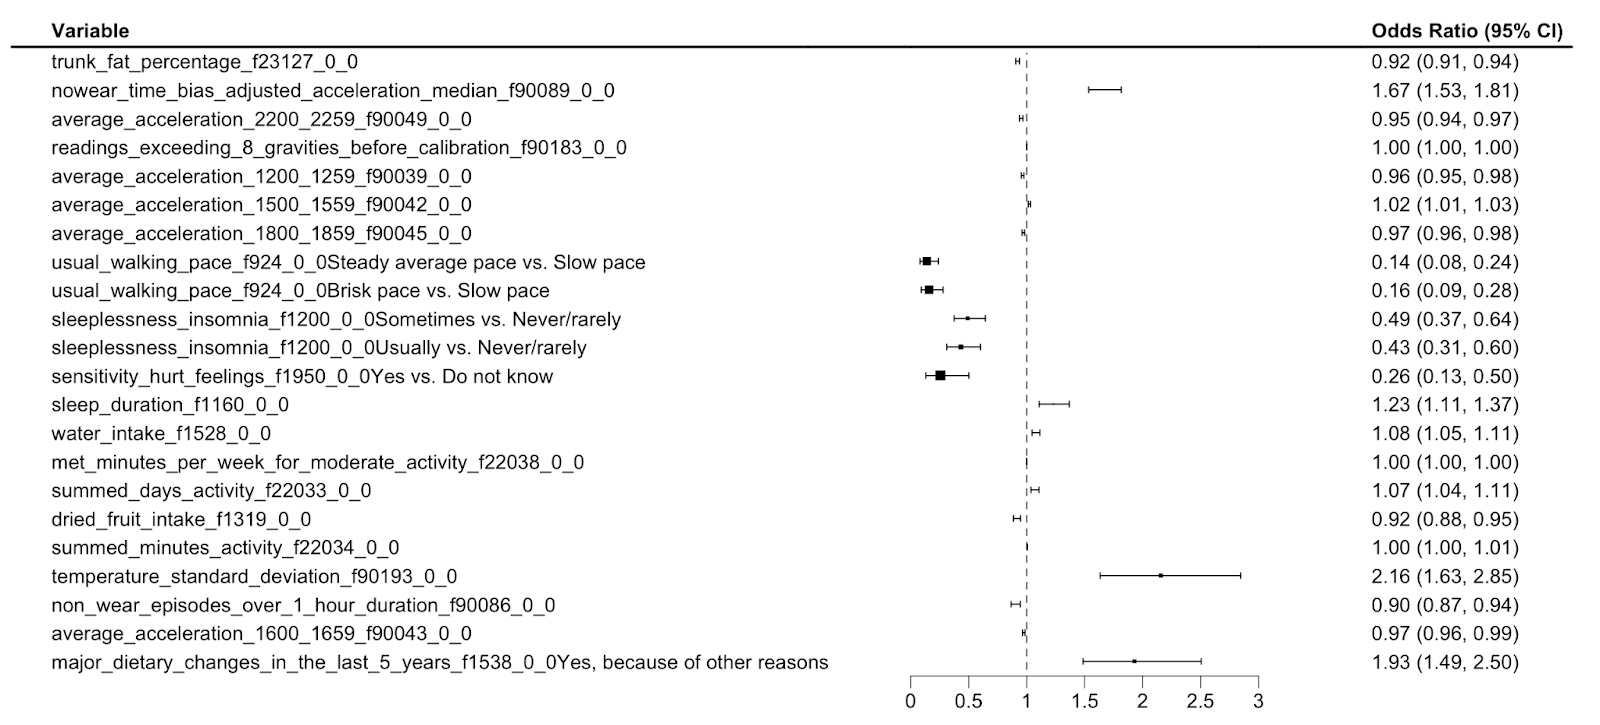
\includegraphics{../figure/Figure 2 - Odds Ratio of PD for Statistically Significant Variables.png}
\caption{Odds Ratio of PD for Statistically Significant Variables}
\end{figure}

In conclusion, our modeling results generally align with existing
literature, suggesting that decreased physical activity, irregular or
unhealthy dietary habits, sleep disorder, and mental health challenges
could serve as potential PD risk factors or early indicators. These
characteristics were statistically significant in distinguishing between
healthy individuals and those who would later develop PD. However, the
mechanism between insomnia and PD onset may require more in-depth
investigation.

\hypertarget{limitations}{%
\subsubsection{Limitations}\label{limitations}}

Our study's analytical model presents several limitations that may
impact the interpretation and generalizability of the findings.
Primarily, our use of logistic regression assumes linear relationships
between the predictors and the log odds of developing Parkinson's
disease, potentially overlooking nonlinear interactions such as
quadratic or interaction effects that might better explain the data.
Alternative feature selection methods like Lasso or Elastic Net, which
provide regularization to manage multicollinearity and reduce the risk
of overfitting, were not employed but could potentially enhance the
robustness of our model. Moreover, the absence of data on other
comorbidities such as diabetes or anemia presents a significant
limitation. These conditions might confound the relationships between
identified risk factors and Parkinson's disease, as they may
independently or synergistically influence PD symptom manifestation.

\hypertarget{task-2---analyze-longitudinal-trends-following-pd-diagnosis}{%
\subsection{Task 2 - Analyze longitudinal trends following PD
diagnosis}\label{task-2---analyze-longitudinal-trends-following-pd-diagnosis}}

\hypertarget{participant-and-feature-selection-1}{%
\subsubsection{Participant and Feature
Selection}\label{participant-and-feature-selection-1}}

Similarly, we began with the full dataset comprising 96,512 participants
and 1,294 features. Of these, 92 participants, out of 463 with PD, had 4
instances recorded after PD reporting, while 96,049 participants had no
such diagnosis. The low prevalence of PD in our dataset presented a
significant challenge due to data imbalance. To address this issue, we
applied propensity score matching, selecting a subset of non-PD samples
that closely matched the demographic profiles (age, sex, ethnicity, and
Townsend index for socioeconomic status) of PD patients. This process
resulted in a balanced cohort of 184 participants, half diagnosed with
PD.

In the next stage of our analysis, we focused on refining feature
selection. We limited our feature set to those that are numeric and have
records across all 4 instances. It is important to note that there were
still some missing values within these 4 instances. This approach helped
us identify 81 unique features, each consistently recorded across four
instances, in addition to the 4 demographic features used in our
matching process.

\begin{figure}
\centering
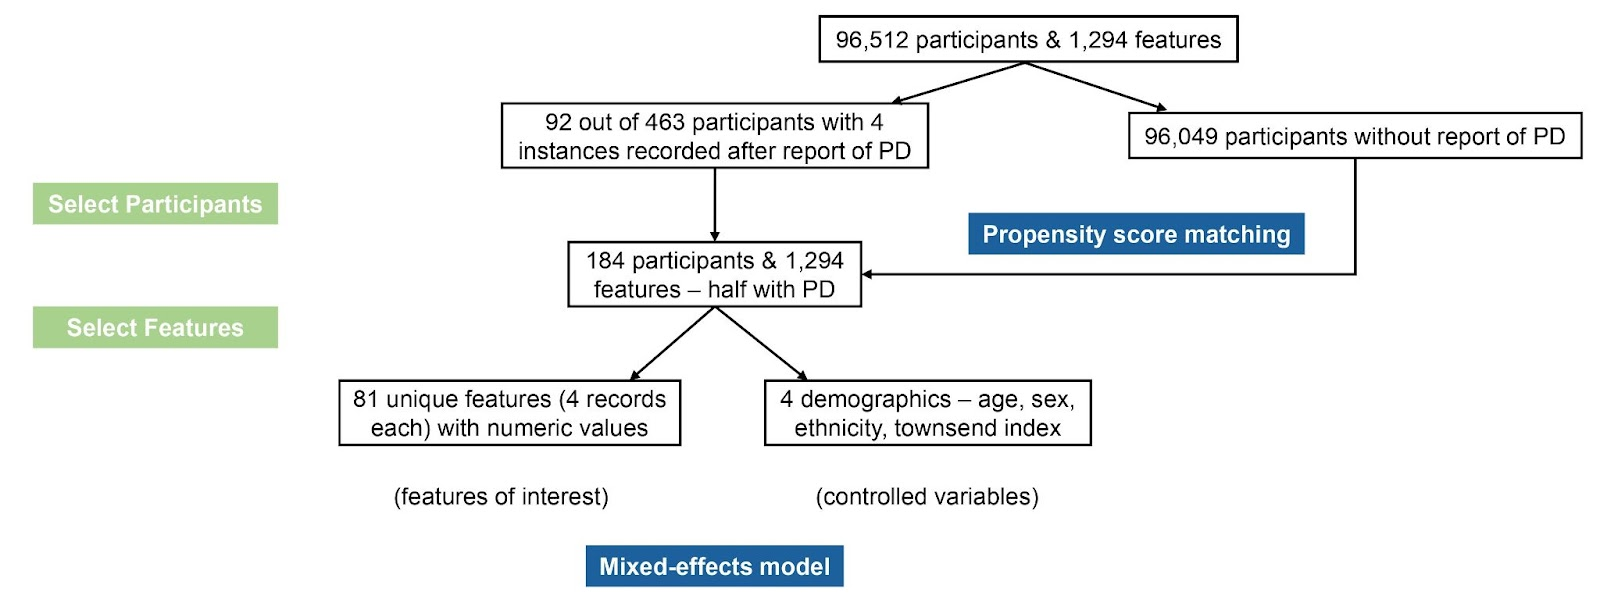
\includegraphics{../figure/Figure 3 - Workflow of Aim 1 - Task 2.png}
\caption{Workflow of Aim 1 - Task 2}
\end{figure}

\hypertarget{mixed-effects-model}{%
\subsubsection{Mixed-effects Model}\label{mixed-effects-model}}

We used linear mixed-effects models (nlme) to assess the differences in
the trends between the group with and without PD. The 4 demographic
variables (age, sex, ethnicity, and Townsend index) were controlled as
fixed effects, participant eid was treated as a random effect, and a
quadratic spline was applied to the time component. We conducted
likelihood ratio tests to evaluate if the average trend and the
interaction between the group and time were significantly different.

\hypertarget{results}{%
\subsubsection{Results}\label{results}}

In the left panel of Figure 4, we retain numeric features that are
significant either at baseline or through interaction effects. We
observe significant differences between the PD and non-PD groups in
terms of baseline for time spent using the computer, sleep duration,
longest period of depression, and average weekly red wine intake.
Specifically, physical symptoms like tremors, rigidity, and restlessness
can make it difficult for PD patients to find a comfortable sleeping
position. Since sleep plays a crucial role in neurodegenerative
disorders, effective management of sleep can enhance quality of life and
provide insights into integrating sleep therapy into care plans for PD
patients. Additionally, the interaction over time for computer usage,
sitting height, and average weekly fortified wine intake shows
significant differences between the two groups. In the right panel, we
visualized the longitudinal trends across 4 instances for some selected
significant features.

\begin{figure}
\centering
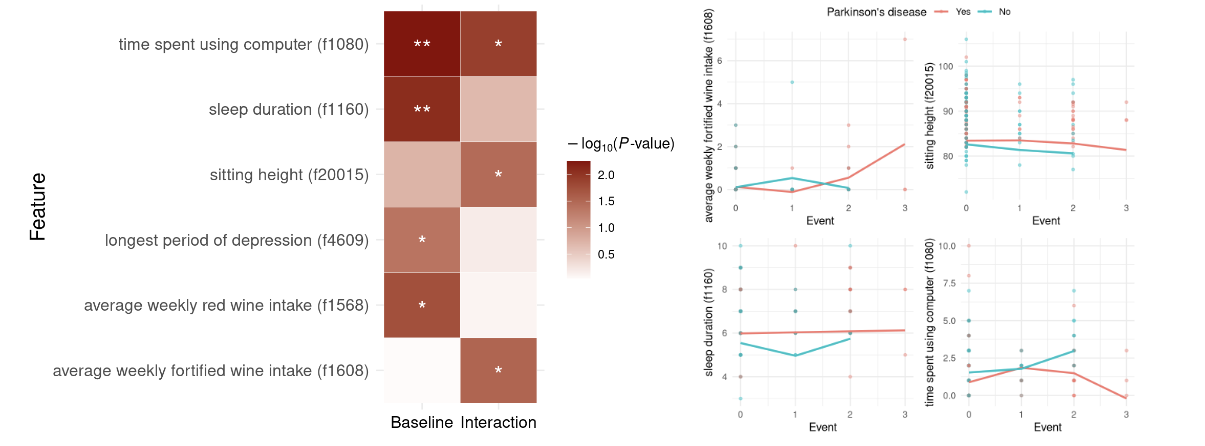
\includegraphics{../figure/Figure 4 - Visualization of Longitudinal Trends.png}
\caption{Visualization of Longitudinal Trends}
\end{figure}

\hypertarget{limitations-1}{%
\subsubsection{Limitations}\label{limitations-1}}

First, there is still a high level of missingness in our small cohort,
which could compromise the accuracy of our model fit. Missing values,
which may stem from refusal to answer, lack of knowledge, or
non-collection, might be disproportionately distributed across PD and
non-PD groups and introduce bias. Second, our current methodology does
not allow us to examine the collective association between the features
of interest within a single model. A potential direction for future
research could be to incorporate methods that address this limitation of
association.

\hypertarget{specific-aim-2-build-practical-and-interpretable-models-for-predicting-the-risk-of-parkinsons-disease-for-each-specific-patient.}{%
\section{Specific Aim 2: Build practical and interpretable models for
predicting the risk of Parkinson's disease for each specific
patient.}\label{specific-aim-2-build-practical-and-interpretable-models-for-predicting-the-risk-of-parkinsons-disease-for-each-specific-patient.}}

\hypertarget{hypothesis-1}{%
\subsection{Hypothesis}\label{hypothesis-1}}

While no definitive cause has been identified in previous studies,
Parkinson's disease is widely believed to be associated with a
combination of various risk factors, including basic demographic
information, environmental risk factors, lifestyle, and family history
of related syndromes. Based on preliminary studies and recognized
literature conclusions, we believe that predicting the risk of
Parkinson's disease, which would significantly contribute to the early
detection of the disease, is both feasible and practical.

For aim 2, we will focus on building a predictive model for each
specific patient to estimate the risk of Parkinson's disease at an
individual level. During this part, we will explore more complex machine
learning methods that differ from traditional statistical models, while
ensuring the simplicity and interpretability of the prediction process.
Furthermore, based on the interpretable trained model, we will also
explore additional indicators that may not be causative but could still
assist in the early diagnosis of Parkinson's disease, further verifying
and supplementing our conclusions from aim 1.

\hypertarget{rationale-2}{%
\subsection{Rationale}\label{rationale-2}}

Contribute to Early Detection: Build a predictive model to estimate the
risk of Parkinson's disease is crucial for early detection and treatment
of the disease. On the one hand, early treatment can help control the
progression of the disease, leading to an improvement in long-term life
quality; On the other hand, Parkinson's disease is associated with
various complications such as postural instability, motor impairments,
and cognitive impairment. Early detection of the disease could
significantly reduce the risk introduced by these complications.

Practical and Cost-efficient: Although genetic factors are recognized as
a crucial component of early Parkinson's diagnosis, conducting tests for
certain genetic mutations always increase the complexity and cost of
detection, making it impractical in wide use. Based on that, we will not
include features related to genetics for aim 2, differing from various
previous studies. Instead, we will focus on achieving more accurate
predictions using other features that are easier to detect and collect.
Additionally, we will also pay attention to the balance between the
model performance and the simplicity of the data processing and
modeling, aiming at building a practical, cost-efficient and widely
applicable model for risk estimation.

Provide Insights for Risk Factors: In contrast to aim 1, aim 2 will
involve modeling the relationship between features and the risk of
Parkinson's disease using more complex tree-based methods. While
ensuring the interpretability, we will also explore various
preprocessing techniques for the original variables, including WOE
binning, information value and NMS algorithm for mitigating
collinearity. With a processing structure different from traditional
statistical methods, models here will provide special insights into the
potential risk factors associated with Parkinson's disease and further
validate the conclusions drawn in aim 1.

\hypertarget{experimental-approach}{%
\subsection{Experimental approach}\label{experimental-approach}}

\begin{enumerate}
\def\labelenumi{\arabic{enumi}.}
\item
  \textbf{1. Basic Data Preparation}

  Basic data preparation would be conducted first to ensure data
  quality:

  \begin{itemize}
  \tightlist
  \item
    Data cleaning: Keep cases which are diagnosed after enrolment
    (incident cases),and if an instance has multiple measurement
    results, compute the average value. Also, compute the difference
    between each measurement and the previous one (first-order
    differencing) to reduce the influence of unexpected fluctuations.
  \item
    Remove columns with missing proportions exceeding 80\%: Features
    with high proportion of missing may not be adequately represented in
    the minority class, while imputation will introduce significant bias
    and make the modeling even more challenging.
  \item
    Drop features with approximately constant values: For categorical
    variables, assess the proportion of different levels. If a single
    level accounts for over 99\% of the samples, it may lack significant
    discriminative ability and can be dropped.
  \end{itemize}

  \textbf{2. WOE + information value for feature filtering}

  WOE (weight of evidence) is a supervised coding methods which is
  commonly used in financial risk models. With tree-based binning, WOE
  values could be calculated for each group to represent the difference
  between ``the proportion of the target customers in the current group
  to all target customers'' and ``the proportion of non-target customers
  in the current group to all non-target customers'': \[
  WOE_{i} = \ln{\frac{y_i/y_T}{n_i/n_T}}
  \] Based on the WOE values for each bin, we can calculate the
  Information Value (IV) as a measure of feature importance: \[
  IV_i = ( py_i - pn_i )*\text{WOE}_i; \quad py_i=\frac{y_i}{y_T},\,\,\,pn_i=\frac{n_i}{n_T}
  \] For aim 2, IV is used as feature filtering, that we set the
  threshold of IV to 0.1 and discard any features with an IV lower than
  this threshold. Binning the numerical variable helps the tree-based
  model converge more efficiently when finding the optimal splitting
  value, making it a suitable feature engineering method based on the
  characteristics of our predictive model (random forest); Moreover, it
  contributes significantly to reducing the model's complexity as a
  feature filter, while also plays a crucial role in other feature
  engineering process, such as dealing with collinearity.

  \textbf{3. NMS algorithm for collinearity problem}

  Given the large number of features in the original dataset (1295),
  severe collinearity poses a significant challenge to further modeling
  and increases the time required to identify an optimal subset of
  features. We employ the Non-Max Suppression (NMS) algorithm as a basic
  solution structure for collinearity. This algorithm, commonly used in
  computer vision, selects a sub-optimal subset of features as follows:

  \begin{enumerate}
  \def\labelenumii{\arabic{enumii}.}
  \item
    Assume the original feature set as \(A\).
  \item
    Select the feature with the highest feature importance (information
    value) and add it to the final feature set \(S\).
  \item
    Calculate the correlation of the chosen feature with every other
    remaining feature in \(A\). Remove features with a correlation
    higher than a threshold (0.8) from \(A\) as redundancy.
  \item
    Select the feature with the second-highest feature importance among
    the remaining features in \(A\), add it to the final feature set
    \(S\), and repeat the steps above.
  \item
    Repeat the process until the remaining feature set \(A\) is empty.
  \end{enumerate}

  With the NMS algorithm, we identified and dropped about 13\% redundant
  variables highly collinear with other more important features. In
  model comparison, we will further validate the effectiveness of the
  NMS method, as models with collinearity processing perform better than
  the original one in terms of recall.

  \textbf{4. Propensity Score Matching}

  Due to the low prevalence of Parkinson's disease within the
  population, we are facing severe data imbalance problem when building
  a classification model. Traditional solution for imbalance including
  subsampling and generating new data with methods such as SMOTE.
  However, considering the characteristics of our dataset, subsampling
  may result in unacceptable information loss, while generating new data
  could make the classification boundary even more ambiguous.

  Given these considerations, propensity score matching (PSM) would be
  used for addressing the imbalance problem. PSM aims to identify a
  subset among non-diseased samples that is most similar to the patients
  with Parkinson's. We believe that it could help construct a dataset
  that is more concentrated around the classification boundary, which
  would significantly contribute to the model in learning and
  characterizing sample features effectively.

  \textbf{5. Predictive Model with Random Forest}

  With the matched data, random forest would be used for building the
  predictive model. As a tree-based model with bagging structure, random
  forest strikes a good balance between model performance and
  complexity. While utilizing nonlinear meta-learners (in this case,
  CART trees) to fit the data, it effectively controls potential
  variance through ensemble learning at the same time, which helps
  mitigate the risk of overfitting.

  We conduct model evaluation with 10-fold cross validation to assess
  the model performance. Meanwhile, several further experiments for
  model comparisons are conducted to further validate the previous
  feature engineering processes.
\end{enumerate}

\hypertarget{results-1}{%
\subsection{Results}\label{results-1}}

The data processing and model construction methods have been outlined
above. Using 742 samples (371 incident cases and 371 matched
non-Parkinson's samples) and 221 features, the following statistical
analyses were conducted in R 4.2.2.

The model performance, assessed with 10-fold cross-validation, is as
follows:

\begin{longtable}[]{@{}llll@{}}
\toprule\noalign{}
recall & AUC & accuracy & F1-score \\
\midrule\noalign{}
\endhead
\bottomrule\noalign{}
\endlastfoot
0.562 & 0.546 & 0.501 & 0.517 \\
\end{longtable}

From the results above, the recall reaches 0.562 with an AUC of
approximately 0.546. Recall is considered a more crucial indicator here
because missing patients with a high risk of Parkinson's could lead to
significant consequences.

On the one hand, diagnosing Parkinson's disease remains challenging
based on preliminary studies. On the other hand, due to the utilization
of propensity score matching, our model is built on a subset of the
dataset that represents the most challenging scenarios (a subset of
non-disease samples that are closest to the classification boundary). We
believe that the model's performance is acceptable under these
considerations.

Furthermore, to validate the effectiveness of the previous feature
engineering process, we conducted a series of experiments using
different model settings for comparison.The baseline setting refers to
using the original dataset without feature filtering but with imputation
for missing values. The second setting, denoted as ``+IV,'' represents
the model with data after information value (IV) filtering but without
collinearity processing (NMS algorithm). The third setting, labeled as
``+IV + NMS,'' reflects the final model setting described in the
experimental approach section. All comparisons are based on the recall
score from 10-fold cross-validation. The results of the model comparison
are as follows:

\begin{longtable}[]{@{}llll@{}}
\toprule\noalign{}
& Baseline & + IV & +IV + NMS \\
\midrule\noalign{}
\endhead
\bottomrule\noalign{}
\endlastfoot
\textbf{recall} & 0.487 & 0.504 & 0.562 \\
\end{longtable}

The final model setting, which incorporates both IV filtering (with WOE
binning) and collinearity processing (NMS algorithm), achieved the
highest score in terms of recall. This demonstrates that these feature
engineering techniques are effective in improving the model performance.

\hypertarget{conclusion}{%
\section{Conclusion}\label{conclusion}}

In the analysis of data pertaining to Parkinson's disease, several
primary factors significantly impacting the likelihood of disease
development have been identified. These factors include sleep disorders,
feelings of nervousness, a slow walking pace, and chest pain. Crucial
numeric features that have demonstrated significant differences at
baseline or through interaction effects, such as time spent using a
computer, sleep duration, the longest period of depression, and average
weekly red wine intake, were retained in our study. Furthermore,
interaction effects over time were notably significant for features like
computer usage, sitting height, and fortified wine intake,
differentiating between Parkinson's disease (PD) and non-PD groups.

These results have been further supported by visualizations of
longitudinal trends for a subset of significant features over four
instances. Physical activity measurements, in particular abnormalities
in movement such as average acceleration and muscle condition indicators
like leg and arm fat-free mass, were highlighted by the tree-based
model's feature importance analysis as being crucial for the early
diagnosis of Parkinson's disease. These measures are consistent with
established early markers of Parkinson's disease, highlighting their
importance in the categorization of the illness.

However, several limitations were encountered in our methodological
approach. The small sample size of PD patients due to data imbalance
poses challenges in assessing the robustness of our models. Furthermore,
the elimination of redundant variables and the application of Weight of
Evidence (WOE) techniques to handle missing values lacked rigorous
validation, which resulted in residual collinearity in the model. It is
impossible to rule out the possibility of less-than-ideal results, even
when the NMS algorithm is used to reduce collinearity. The random forest
model's insensitivity to collinearity is advantageous, but it could
perform better with more thorough data preprocessing.

In conclusion, this study illustrates the complex nature of diagnosing
Parkinson's disease, emphasizing both the important markers and the
methodological nuances of predictive modeling. Our research facilitates
early detection of Parkinson's disease to slow its progression and
increase intervention opportunities, while also potentially developing
preventive public health initiatives by identifying lifestyle factors
associated with the disease to reduce its overall incidence.

\hypertarget{references}{%
\section{References}\label{references}}

National Institute of Neurological Disorders and Stroke. (2023, January
30). Parkinson's Disease: Challenges, Progress, and Promise. Accessed
February 21, 2024. Mayo Clinic. (2023, May 26). Parkinson's Disease.
Accessed February 21, 2024. UK Biobank. (n.d.). What is UK Biobank?
Accessed February 21, 2024. National Institute on Aging. (2022, April
14).

Parkinson's Disease: Causes, Symptoms, and Treatments. Accessed February
21, 2024. UK Biobank. (n.d.). View the Data Showcase. Accessed February
21, 2024. \url{https://biobank.ctsu.ox.ac.uk/crystal/} Park, H. A., \&
Ellis, A. C. (2020). Dietary Antioxidants and Parkinson's Disease.
Antioxidants (Basel), 9(7), 570.
\url{https://doi.org/10.3390/antiox9070570}

Zuzuárregui JRP, During EH. Sleep Issues in Parkinson's Disease and
Their Management. Neurotherapeutics. 2020;17(4):1480-1494.
\url{doi:10.1007/s13311-020-00938-y}.
\url{https://www.ncbi.nlm.nih.gov/pmc/articles/PMC7851262/}

Gjerstad MD, Wentzel-Larsen T, Aarsland D, Larsen JP. Insomnia in
Parkinson's disease: frequency and progression over time. J Neurol
Neurosurg Psychiatry. 2007;78(5):476-479.
\url{doi:10.1136/jnnp.2006.100370}.
\url{https://www.ncbi.nlm.nih.gov/pmc/articles/PMC2117851/}

Santiago JA, Bottero V, Potashkin JA. Biological and Clinical
Implications of Comorbidities in Parkinson's Disease. Front Aging
Neurosci. 2017;9:394. Published 2017 Dec 4.
\url{doi:10.3389/fnagi.2017.00394}.
\url{https://www.ncbi.nlm.nih.gov/pmc/articles/PMC5722846/}

Chairta, P. P., Hadjisavvas, A., Georgiou, A. N., et al.~(2021).
Prediction of Parkinson's Disease Risk Based on Genetic Profile and
Established Risk Factors. Genes (Basel), 12(8), 1278.
\url{https://doi.org/10.3390/genes12081278}

Yoon, S. Y., Park, Y. H., Lee, H. J., Kang, D. R., \& Kim, Y. W. (2022).
Lifestyle Factors and Parkinson Disease Risk: Korean Nationwide Cohort
Study With Repeated Health Screening Data. Neurology, 98(6), e641-e652.
\url{https://doi.org/10.1212/WNL.0000000000012942}

\bibliography{references.bib}


\end{document}
